\section{The SOLAR-H Structure--Temperature Decomposition Model}\label{sec:solar-method}

\subsection{Design Motivation}

In physical chemistry, dissolution is governed by solid--liquid equilibrium thermodynamics. The classical van 't Hoff equation ties the molar solubility to temperature through the apparent enthalpy of dissolution:
\begin{equation}
\frac{\partial \ln S}{\partial (1/T)} = -\frac{\Delta H_{\mathrm{sol}}}{R}.
\end{equation}
Over a limited operating window, a first-order Taylor approximation implies that the log-solubility depends quasi-linearly on the temperature displacement from a reference point. More importantly, $\Delta H_{\mathrm{sol}}$ is set by the difference between the solute--solvent solvation forces and the solute lattice energy, and is therefore strongly structure-specific.

A conventional regressor that feeds temperature in as one column among many molecular features confuses temperature variation with the absolute solubility differences between parents---temperature occupies only one dimension and each combination is measured over a different range---so the learned temperature response drifts badly on unseen parents. SOLAR-H (Structured Orthogonal Linear \& Additive Regression -- Hybrid) decouples the two: the local temperature slope is estimated orthogonally from within-combination temperature variation, and a tree ensemble then fits the structural baseline on a temperature-corrected target.

\subsection{Structure--Temperature Decomposition}

For the $i$-th record's combination $c_i$, we extract 11 base physicochemical descriptors for the drug and the solvent (molecular weight, MolLogP, TPSA, hydrogen-bond donors/acceptors, aromatic-ring count, and so on), standardise them per training fold, and form a 44-dimensional structural vector $z_c$ that combines the raw values, the Hadamard products, and the absolute differences. Adding a bias term gives the augmented vector $u_c = [1; z_c] \in \mathbb{R}^{45}$.

The temperature is robustly standardised with the training median $T_0$ and interquartile range $s_T$:
\begin{equation}
\tau_i = \frac{T_i - T_0}{s_T}.
\end{equation}
SOLAR-H expresses the predicted log-solubility as an additive combination of a structural baseline and a temperature response:
\begin{equation}\label{eq:v2-solar}
\widehat y_i = b(z_c) + \gamma \cdot \tau_i \cdot \left( u_c^\top \beta \right),
\end{equation}
where $b(z_c)$ is the nonlinear structural baseline at the reference temperature ($\tau_i = 0$, i.e.\ $T_i = T_0$) fitted by ExtraTrees, $u_c^\top \beta$ the local temperature slope of combination $c$, $\beta \in \mathbb{R}^{45}$ the structural modulation coefficients, and $\gamma \in [0, 1]$ the global temperature-gain shrinkage.

\subsection{Within-Group De-meaning Estimation}

The hard part is that the unknown baseline $b(z_c)$ is highly nonlinear; optimising it jointly would let the enormous absolute solubility differences between molecules swamp $\beta$.

SOLAR-H therefore borrows the fixed-effects device from panel-data econometrics. For each training combination $c$ with at least two distinct temperatures, define the within-group means $\bar y_c = \frac{1}{|c|}\sum_{i \in c} y_i$ and $\bar\tau_c = \frac{1}{|c|}\sum_{i \in c} \tau_i$, and subtract them inside each combination:
\begin{equation}
(y_i - \bar y_c) = \left[ b(z_c) - b(z_c) \right] + \gamma (u_c^\top \beta) (\tau_i - \bar\tau_c) + (\varepsilon_i - \bar\varepsilon_c).
\end{equation}
The unknown nonlinear baseline $b(z_c)$ cancels exactly. With the demeaned label $\Delta y_i = y_i - \bar y_c$ and the demeaned feature vector $A_i = (\tau_i - \bar\tau_c) u_c^\top \in \mathbb{R}^{45}$, and under the base gain $\gamma = 1$, estimating $\beta$ reduces to a parent-weighted ridge regression with $\ell_2$ regularisation:
\begin{equation}
\widehat\beta = \arg\min_\beta \sum_{i: |\Delta\tau_i| > 0} w_i(q=1) (\Delta y_i - A_i \beta)^2 + \lambda \|\beta\|_2^2.
\end{equation}
Setting the gradient to zero gives the closed form
\begin{equation}
\widehat\beta = (A^\top W A + \lambda I)^{-1} A^\top W \Delta y,
\end{equation}
where $W$ is the diagonal matrix of parent-equal weights $w_i(q=1)$ (Eq.~\eqref{eq:v2-train-weight}) and $\lambda$ the ridge penalty (fixed at 1000 for numerical stability of the inverse). Because the estimator strips away the absolute solubility differences between parents and uses only the temperature-driven within-system variation, it recovers the physical temperature effect without bias.

\subsection{Structural Baseline and Joint Fitting}

Once $\widehat\beta$ is available, the temperature contribution of every training sample is $\widehat\delta_i(\gamma) = \gamma \tau_i u_c^\top \widehat\beta$, and the corrected structural-baseline target is
\begin{equation}
\widetilde y_i(\gamma) = y_i - \widehat\delta_i(\gamma).
\end{equation}
A parent-weighted ExtraTrees ensemble (200 trees, minimum leaf size 1) is then trained on $\widetilde y_i$ to give $\widehat b(z_c)$. Inside the three-fold nested validation, we grid-search the tree-depth ceiling (8, 16, unbounded) jointly with the temperature gain $\gamma \in \{0, 0.1, 0.3, 1.0\}$, selecting by parent-weighted MAE; the chosen configuration is refit on the outer training set.

\subsection{Ablation and Adaptive Gain}

To isolate the contribution of each SOLAR-H module to cross-parent generalisation, we run a systematic ablation under the outer five-fold cross-validation, holding the parent split, test set, and seeds fixed while toggling parent weighting ($q=0$), the explicit interaction features, the temperature term entirely ($\gamma=0$), and a forced full gain ($\gamma=1$). The results and the paired-bootstrap 95\% intervals appear in Figure~\ref{fig:v2-solar-ablation}.

\begin{figure}[htbp]
\centering
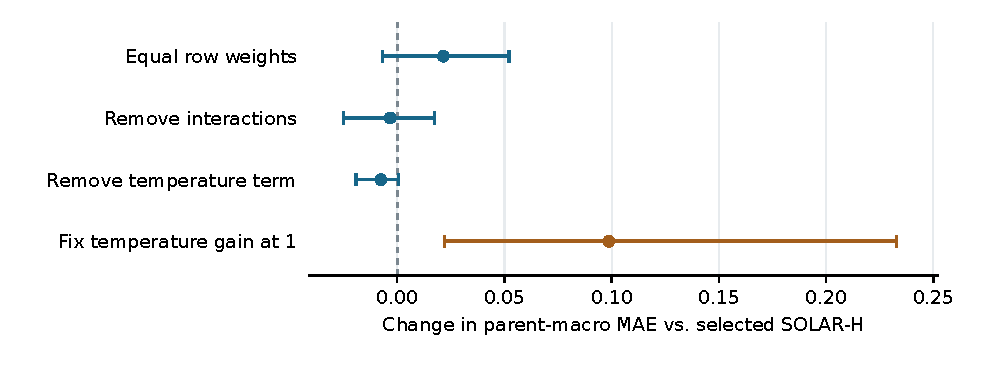
\includegraphics[width=\linewidth]{solar_ablation.pdf}
\caption{Ablation of the core SOLAR-H mechanisms. Points show each configuration's change in parent-weighted MAE relative to the adaptive baseline (positive means larger error); bars are 95\% intervals from 10,000 parent-paired bootstrap resamples.}
\label{fig:v2-solar-ablation}
\end{figure}

The ablation exposes the generalisation mechanism. Turning off parent weighting pushes the MAE on unseen parents to 0.7380 (up 0.0216), confirming that reweighting is what tames the frequent parents and secures the baseline for rare ones. The gain term matters even more: forcing the full gain ($\gamma = 1.0$) sends the MAE to 0.8150 (a deterioration of 0.0987), because the narrow temperature windows of small-sample combinations are easily perturbed by measurement noise; the adaptive shrinkage chosen inside the nested validation ($\gamma \in \{0, 0.1\}$) suppresses this over-extrapolation and keeps the learned temperature response stable.

\subsection{Summary}

This chapter built SOLAR-H, a decomposition that is both thermodynamically interpretable and statistically rigorous: within-group fixed effects remove the structural-baseline confounding, a weighted ridge regression yields a closed-form slope, and the nested validation pins down the adaptive gain. The ablations not only justify each component but also point to a methodological rule---extrapolating a physical slope to unseen scaffolds requires adaptive damping.
